\subsection{The Gust Modeling}

The model which is used in the \emph{flowPsi} to model the gust is call a 
Fiedl Velocity Model, FVM which intriduces gust into \emph{flowPsi} through adding 
artifitial grid velocity
The FVM physically introduces gusts into a CFD code by adding a perturbation velocity\cite{Parameswaran,Singh}
to grid velocity. This perturbation velocity depends on gust shape and its actual position in the domain
in time. The grid however, is stationary, the perturbation velocity is entirely arifitial.  
In \emph{flowPsi} this perturbation velocities are added to the grid cell faces normal velocity component.
The implementation enables to analyze gust while the grid is rigid or moving.  
The gust model which is currently implemented in \emph{flowPsi} is a \emph{1-cos} gust and 
\emph{step} gust.

\subsubsection{\emph{1-cos} Gust}
The \emph{1-cos} gust is a discreet gust which assumes the gust velocities have \emph{1-cos} profile\cite{USDT}.
The equation of  \emph{1-cos} gust is 
\begin{equation}
u_g = \frac{U_{ds}}{2}\Bigg(1-cos\Big(\frac{\pi S}{L}\Big)\Bigg)
\end{equation}
where $U_{ds}$ is the maximum velocity for the gust, $L$ is the gust gradient length 
and $S$ is a gust penetration distance. It is shown in Fig \ref{1-cosgust}
\begin{figure}[htbp]
  \centering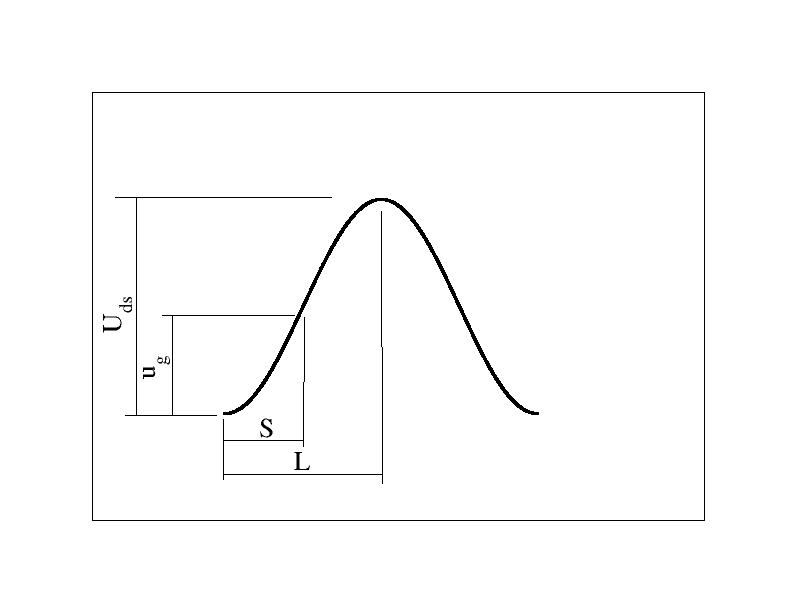
\includegraphics[clip,width=.5\textwidth]{Figures/gust.jpg}
\caption{schematics of \emph{1-cos} gust}\label{1-cosgust}
\end{figure}

\subsubsection{\emph{step} Gust}
Step gust is defined as a sudden change in normal velocity. It then propagates through the computational domain 
at speed and in direction of free stream velocity.
It is shown in Fig \ref{step}
\begin{figure}[htbp]
  \centering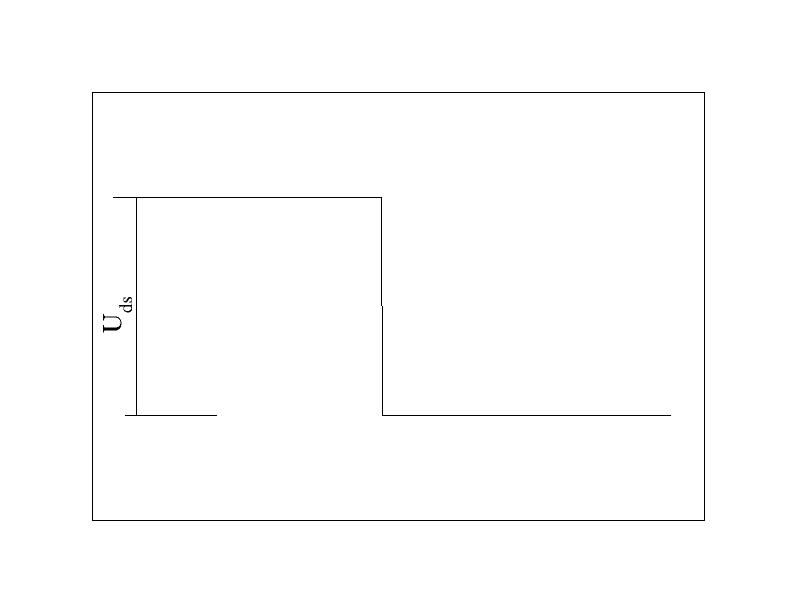
\includegraphics[clip,width=.5\textwidth]{Figures/step.jpg}
\caption{schematics of \emph{step} gust}\label{step}
\end{figure}

\subsubsection{Tabulated Gust}
The gust may be specified by a table. The table is in file which starts with integer number specifying how many 
lines specifying the gust are in the file. This is followed by gust table, see chapter \emph{Gust Specification}.
The name of input file with gust data is specified in \emph{.vars} file.

